\lhead{\emph{Motivación}}
\chapter{Motivación}

\section{Introducción}

Los límites físicos de los que adolecen los computadores en la época actual hacen de la computación distribuida y paralela un método para incrementar de forma sencilla y rentable el rendimiento total de un sistema, rendimiento que aumenta significativamente en problemas \textit{ridículamente paralelos}\citationneeded.

Sin embargo, estas ganancias conllevan una serie de inconvenientes, o el aumento de la complejidad de diversas tareas. En general, un sistema distribuido requiere de un conjunto de máquinas independientes, que en conjunto suelen suponer un coste superior al de un único nodo. Además, aparecen nuevos problemas de índole técnica: problemas de comunicación, integridad y sincronización, dificultad en el desarrollo y depuración de aplicaciones, etcétera.

En el apartado didáctico, el estudio del paradigma distribuido suele requerir un gran esfuerzo por parte de los estudiantes, en particular para comprender los fundamentos básicos de cualquier aplicación distribuida.

\section{Motivación}

El sistema descrito en esta memoria surge inspirado en proyectos similares y se desarrolla con una serie de objetivos claros e independientes:

\begin{itemize}
	\item Como herramienta de síntesis de los conocimientos adquiridos en la carrera, se busca la creación de un sistema completo desde sus cimientos hasta los componentes de más alto nivel, gestionando las tareas de mantenimiento, instalación y manejo del mismo, así como los protocolos de trabajo, tanto en cada uno de los componentes (nodos) como en la comunicación entre los mismos. Con un enfoque más teórico, se pretende crear un sistema capaz de poder ser utilizado como herramienta de diseño y prueba de algoritmos que resuelvan problemas gracias al paradigma de la computación distribuida.
	\item Potenciar el aprendizaje en el mundo de los sistemas operativos, sistemas embebidos, redes de computadores, sistemas distribuidos, administración de sistemas y algoritmos.
	\item Constituir una herramienta didáctica para varias asignaturas cursadas en el plan de estudios del Grado en Ingeniería Informática en la Universidad de Salamanca, analizando las asignaturas relevantes en el Plan y buscando soluciones a las necesidades propuestas por el Profesorado, Estudiantes y Administradores del sistema.
	\item Intentar elevar el \textit{state of the art} en el mundo de los sistemas distribuidos con plataformas embebidas mediante la creación de un sistema multipropósito en lugar de soluciones con un fin determinado.
\end{itemize}

Partiendo de la premisa de las potenciales ventajas del uso de este tipo de computadores en detrimento de otras soluciones se plantea el sistema definitivo.

\section{Objetivos del sistema}

Durante las fases de definición del proyecto, se plantean los siguientes objetivos a cumplir para la consecución del sistema:

\subsection{Diseño y construcción de la arquitectura física del sistema}
Se deberán definir las interconexiones entre los diferentes componentes del sistema, solucionar los diferentes problemas físicos tales como la alimentación eléctrica, conexiones de red, refrigeración\dots analizando los diferentes enfoques y valorando la mejor solución en función del resto de objetivos a cumplir.

\subsection{Gestión del sistema}

El sistema debe contar con un conjunto de herramientas que mantengan los principios de transparencia propios de un sistema distribuido.

\subsection{Integración}
El sistema debe integrarse en una infraestructura preexistente, sin que dicha integración comprometa el diseño básico del sistema, a fin de facilitar su adaptabilidad a otros entornos.

\subsection{Uso como herramienta didáctica}
El sistema debe ofrecer una serie de ventajas a las herramientas didácticas utilizadas en aquellas asignaturas donde se impartan conocimientos relacionados con la computación paralela y distribuida, ofreciendo herramientas que faciliten la comprensión de dichos paradigmas o el desarrollo, prueba y aplicación de programas basados en los mismos.

\subsection{Evaluación}

A fin de probar los objetivos definidos anteriormente, la viabilidad de sistema como herramienta didáctica y su integración en la organización deberán ser determinados por los diferentes usuarios de la misma.


Durante el desarrollo del proyecto surgen los siguientes objetivos funcionales

\subsection{Simplicidad de MarcoPolo}

MarcoPolo debe conseguir un alto grado de versatilidad y aplicabilidad en un gran rango de aplicaciones. A fin de conseguir este objetivo, la simplicidad del sistema construido es clave. Esto conlleva el desacoplamiento y delegación de gran parte de la funcionalidad a otras capas superiores, independientes del protocolo, pero que aprovechan su funcionalidad, en lugar de ser integradas en el mismo.

\subsection{Test-Driven Development}

\section{Conceptos teóricos}

\section{Situación actual (\textit{state of the art})}

%Este apartado sería parecido a lo que en trabajos de grado (WHVLQDV \ WHVLV) se denomina estado del arte. En un proyecto de final de carrera de primer ciclo no parece obligada su presencia (D GLIHUHQFLD GHO VHJXQGR FLFOR GRQGH OD MXVWLILFDFLyQ WHyULFD PHGLDQWH XQ HVWDGR GHO DUWH GHEH DFRPSDxDU D ORV SURGXFWRV VRIWZDUH UHDOL]DGRV), aunque se puede dejar a juicio del tutor o tutores el incluir un pequeño resumen comentado de los trabajos y proyectos ya realizados en el campo del proyecto en curso.

\subsection{Computadores de placa única}

Los computadores de placa única (\textit{Single-Board Computer}) consisten en computadores de generalmente bajas prestaciones que aglutinan todos los componentes necesarios para su funcionamiento en un único circuito integrado. Dichas placas suelen tener un coste bajo y una relación rendimiento/coste muy elevada.

Durante los últimos años se han popularizado como una herramienta para el estudio y creación de sistemas distribuidos con un gran rango de propósitos diferentes.

\subsubsection{RPiCluster (Joshua Kiepert)}

Joshua Kiepert, estudiante de doctorado en la universidad Boise State, crea este sistema utilizando 33 computadores \textbf{Raspberry Pi B}, con el objetivo de utilizarlo como herramienta de pruebas que sirva de alternativa al supercomputador situado en su universidad\cite{joshuarpicluster}, sobre el que trabaja de forma rutinaria, a fin de poder continuar su trabajo en periodos de mantenimiento, cierre del centro, etcétera. El sistema está diseñado para utilizar la \textit{Message Passing Interface} y además poder utilizar los diferentes puertos de las placas (GPIO, I\textsuperscript{2}C, SPI, UART), puertos generalmente ausentes en computadores como clústeres. Utiliza además un servidor \textbf{NFS} para compartir datos entre todos los nodos, y un \textit{router} dedicado para la interconexión. El sistema se complementa con un ordenador \textbf{Chromeboox} con el mismo sistema operativo (\textbf{Arch Linux}), que actúa como nodo coordinador.

%TODO: Diagram here
% http://www.zdnet.com/article/build-your-own-supercomputer-out-of-raspberry-pi-boards/

\begin{figure}[H]
\centering
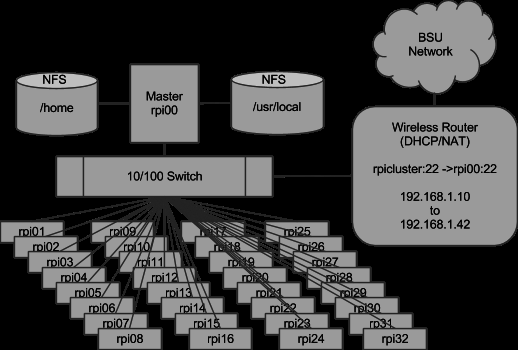
\includegraphics[width=0.5\textwidth]{Chapter1/Figures/structure.png}
\caption{Estructura del sistema (Fuente: Joshua Kiepert).}
\label{kiepert:structure}
\end{figure}

\textbf{Coste}: 1967.21 dólares.


\subsubsection{Dramble (Jeff Geerling)}

El clúster \textit{Dramble} es un conjunto de 6 equipos \textbf{Raspberry Pi} capaces de ejecutar en conjunto el gestor de contenidos \textbf{Drupal}\footnote{\href{https://www.drupal.org/}{drupal.org}}. El sistema es utilizado como servidor de pruebas para la ejecución de instancias de \textbf{Drupal} de forma experimental o durante demonstraciones en público\cite{geerlingraspberry}.

\begin{figure}[H]
\centering
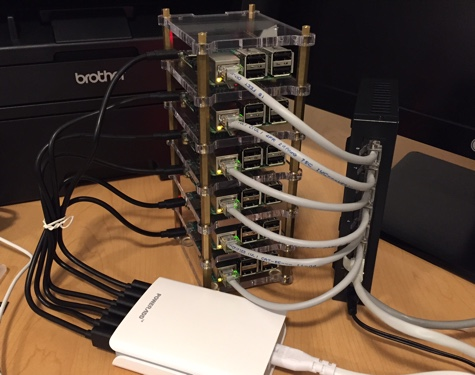
\includegraphics[width=0.5\textwidth]{Chapters/Chapter1/Figures/raspberry-pi-dramble-cluster-wired.jpg}
\caption{El \textit{Dramble} en ejecución}
\label{geerling:dramble}
\end{figure}


\textbf{Coste (estimado)}: 35 dólares por cada Raspberry Pi\citationneeded

\subsubsection{Bramble (GCHQ)}

El organismo gubernamental \textit{Government Communication Headquarters}, agencia de inteligencia del Gobierno Británico presentó en la \textit{Big Bang Fair} de 2015 un proyecto educativo que combina 66 \textit{Raspberry Pi} en un clúster jerárquico con 8 grupos de 8 nodos, cada uno de ellos con un coordinador, y dos nodos coordinadores. El cableado se reduce gracias al uso de la tecnología \textbf{PoE} (\textit{Power over Ethernet}), y cada \textbf{Raspberr} cuenta con un conjunto de elementos adicionales, como un reloj de tiempo real, disco duro externo, cámara, punto de acceso WiFi, etcétera\cite{gchqbramble}.

\begin{figure}[H]
\centering
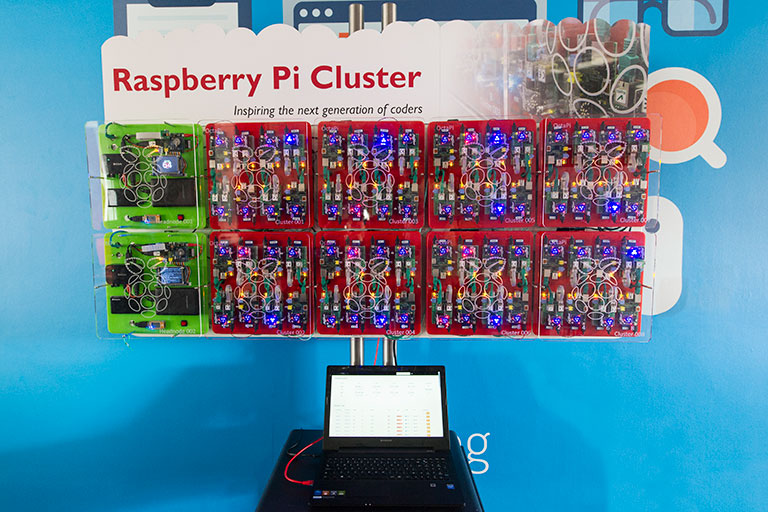
\includegraphics[width=0.5\textwidth]{Chapters/Chapter1/Figures/bramblegchq}
\caption{Vistazo general de la estructura del sistema}
\label{gchq:bramble}

\textbf{Coste (estimado)}\citationneeded

\end{figure}

\subsubsection{Clúster Iridis (Simon Cox, University of Southampton)}

Con el objetivo de atraer a jóvenes estudiantes al mundo de la Computación, el profesor Simon Cox crea este clúster con 64 \textbf{Raspberry Pi B} sobre una estructura de LEGO\cite{cox:raspberry}
%TODO: http://www.i-programmer.info/news/91-hardware/8385-gchq-builds-a-raspberry-pi-cluster.html
\begin{figure}[H]
\centering
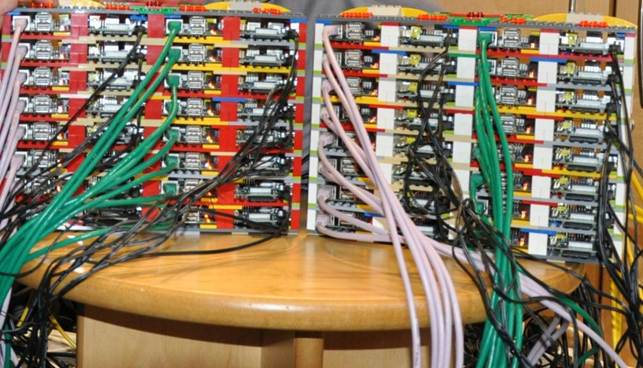
\includegraphics[width=0.5\textwidth]{Chapters/Chapter1/Figures/iridis-pi.jpg}
\caption{Sistema}
\label{cox:iridis}

%w
\end{figure}

\subsubsection{Paralella}

%http://www.zdnet.com/article/parallella-the-99-linux-supercomputer/

%http://www.webstreet.com/super_computer.htm